\section{Experimentation}
\label{sec:experiments}

In this section, we evaluate how adaptiveness of \SPRAY impacts common metrics
of peer sampling performances including clustering coefficient, average
shortest path length, in-degree distribution, arc count, connected
components. We use \CYCLON as baseline with a fixed-size view for experiments
relative to adaptivity. We expect similar behavior when network size is optimal
for \CYCLON. We expect \SPRAY to save resources when \CYCLON is oversized. We
expect \SPRAY to be more robust when \CYCLON is undersized. Finally, we expect
\SPRAY to keep number of duplicates in partial view very low. We use \SCAMP as
baseline for experiments relative to connection failures. We expect \SPRAY to
tolerate connection failures.  We do not use \SCAMP for experiments relative to
adaptivity since SCAMP fails to maintain a random graph in WebRTC context.

\begin{figure*}
  \centering
  \subfloat[Figure A][Clustering coefficient of \CYCLON.]{
    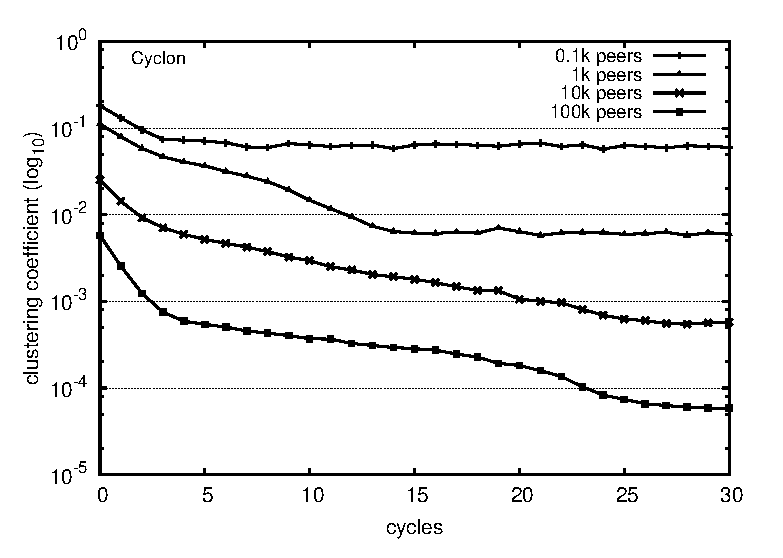
\includegraphics[width=0.45\textwidth]{img/cycloncluster.eps}}
  \hspace{10pt}
  \subfloat[Figure B][Clustering coefficient of \SPRAY.]{
    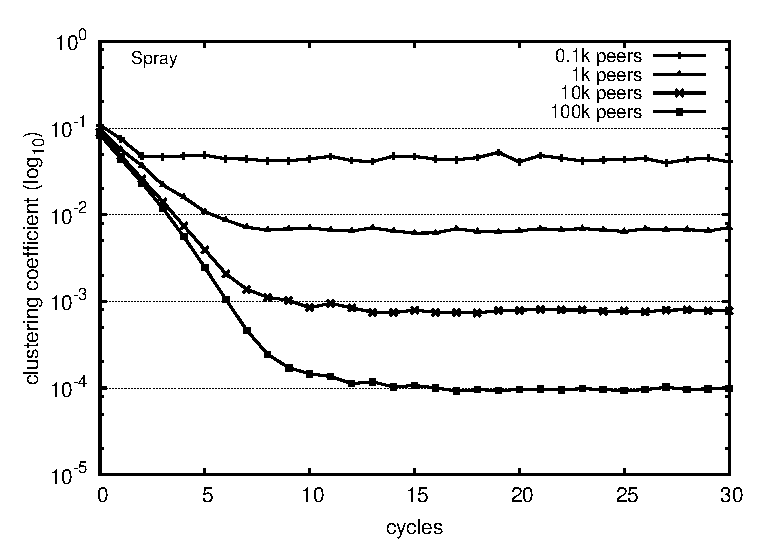
\includegraphics[width=0.45\textwidth]{img/spraycluster.eps}}
  \caption{\label{fig:clustering}The x-axis denotes the elapsed time in cycles
    while the y-axis denotes the $\log_{10}$-scaled clustering coefficient.}
\end{figure*}


The experiments run on the \PEERSIM
simulator~\cite{montresor2009peersim}. The code of the random peer sampling
protocols \CYCLON, \SCAMP, and \SPRAY is available on the Github
platform\footnote{\url{https://github.com/justayak/peersim-spray}}.

\subsection{Clustering coefficient}
\label{subsec:cluster}

% \begin{figure}
%   \centering
%   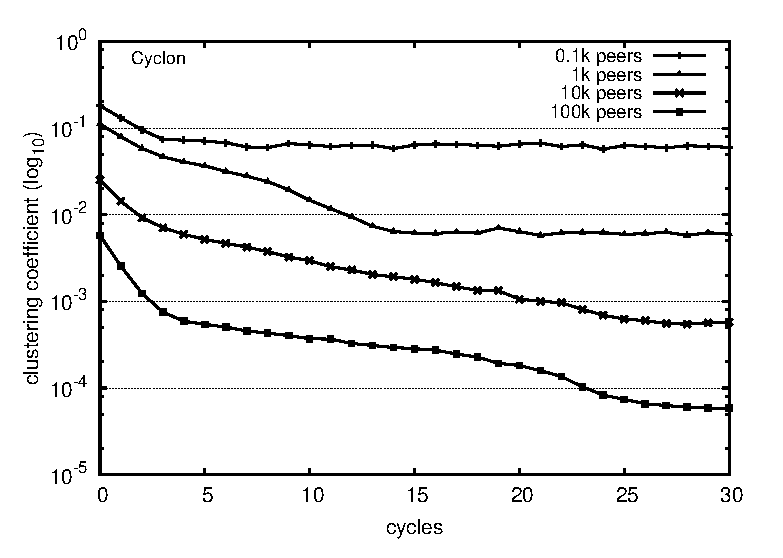
\includegraphics[width=0.49\textwidth]{img/cycloncluster.eps}
%   \caption{\label{fig:clustering}The clustering coefficient of \CYCLON and
%     \SPRAY: the x-axis denotes the elapsed time in cycles while the y-axis
%     denotes the $\log_{10}$-scaled clustering coefficient.}
% \end{figure}

\begin{asparadesc}
\item[Objective:] To observe how adaptiveness impacts on clustering and
  convergence speed.
\item[Description:] The average clustering coefficient $\overline{C}$ measures
  the connectivity of each peer's neighborhood in the network.
  \begin{equation}
    \overline{C} = {1\over |\mathcal{N}|}\sum\limits_{x\in\mathcal{N}}C_x
  \end{equation}
  where $C_x$ is the local clustering coefficient of Peer $p_x$.  The runs
  concern 0.1k, 1k, 10k and 100k peers. The representative of fixed-size
  approach is \CYCLON which is optimally configured for 1k peers. Indeed, its
  partial views are set to $\ln(1000)\approx 7$ neighbors. During their
  exchange, the peers using \CYCLON shuffle $3$ out of their $7$
  neighbors. Thus, \CYCLON is oversized for 0.1k peers and undersized for 10k
  peers and 100k peers.
\item[Results:] Figure~\ref{fig:clustering} shows that \CYCLON starts with a
  lower clustering coefficients than \SPRAY. Still, \SPRAY converges faster
  than \CYCLON. Furthermore, when the number of peers in the network grows, the
  convergence speed of \CYCLON suffers heavily. On the contrary, \SPRAY
  converges very quickly independently of the network
  size. Figure~\ref{fig:clustering} also shows that both the approaches
  converge to a low clustering coefficient which is characteristic of random
  graphs. Nevertheless, \CYCLON and \SPRAY do not raise the same values after
  convergence. Indeed, excepted the number of peers where \CYCLON is optimally
  configured, \SPRAY's values are either below (when \CYCLON is oversized) or
  above (when \CYCLON is undersized).  Overall, it shows that \SPRAY is
  \begin{inparaenum}
  \item faster to converge to a clustering coefficient
  \item reflecting the needs of the network membership.
  \end{inparaenum}
  It impacts both load-balancing and robustness to churn (when peers join and
  leave the network freely).
\item[Reasons:] \CYCLON starts with a lower clustering coefficient because each
  peer performs random walks to advertise themselves in the network. Hence, the
  starting overlay is already slightly balanced when the simulation starts the
  shufflings. On the other hand, a newcomer peer in \SPRAY only advertise
  itself to the neighborhood of its contact peer. Therefore, the network
  overlay starts strongly unbalanced, independently of the network size. Still,
  \CYCLON converges slower than \SPRAY because of its fixed-size partial view
  and the size of the shuffle. When they are \emph{a priori} configured, they
  constitute a constraint to the convergence speed.  The clustering coefficient
  measures how much the neighborhood of each peer is connected to the rest of
  the network. It directly depends of the partial view size of each peer which,
  in \CYCLON, is fixed. Thus, when the peers number is multiplied by $10$, the
  clustering coefficient after convergence is divided by $10$. On the other
  hand, the peers using \SPRAY have variable-size partial view which gently
  reflects the network size with a logarithmic growth. Thus, when the network
  has 1000 peers, the partial view size adapts to this network size. It
  explains the slightly lower clustering coefficient of \SPRAY on this run
  (\SPRAY 7.4 vs \CYCLON 7). By extending the reasoning, it explains the
  reasons of the \SPRAY lower value when \CYCLON is oversized, and the reasons
  of the \SPRAY higher value when \CYCLON is undersized.
\end{asparadesc}

\subsection{Average shortest path length}
\label{subsec:avg}

\begin{asparadesc}
\item[Objective:] To observe how adaptiveness impacts on the average shortest
  path length, i.e., on the efficiency of information dissemination.
\item[Description:] The average path length is the average of the shortest path
  length between peers in the graph. It counts the minimum number of hops to
  reach a peer from another given peer. It basically represents the traveling
  time of any information to reach all the peers at least once. We average the
  path length on a small subset of the network membership and run $100$ times
  the simulation on \SPRAY to avoid any side effects due to randomness. We also
  run the simulation on different configurations of \CYCLON targeting different
  optimal network size. \CYCLON set with the partial view size of 7 roughly
  targets 1.1k peers. \CYCLON set with the partial view size of 9 roughly
  targets 8.1k peers. \CYCLON set with the partial view size of 11 roughly
  targets 60k peers. In all these simulations, we perform the measurements
  after convergence. The checkpoints for the measurements are 0.1k, 0.5k, 1k,
  5k, 10k, 50k, and 100k peers.
\item[Results:] Figure~\ref{fig:avgpath} shows that both \CYCLON and \SPRAY
  have an average shortest path length relatively small. Thus, the information
  can disseminate to all the network very quickly. Figure~\ref{fig:avgpath}
  also shows that, each run of \CYCLON taken alone can be divided in three
  parts compared to \SPRAY. First, an oversized \CYCLON disseminates the
  information faster than \SPRAY. Then, \SPRAY and \CYCLON are equivalent
  where the latter is optimally configured. Finally, \SPRAY yields better
  results. Yet, overall, \SPRAY scales better than \CYCLON since the
  gradient of the former is lower than any configuration of the latter one.
\item[Reasons:] We perform all the measurements after convergence where the
  network overlay is closely related to random graphs. In such graph, the
  diameter and average shortest path length stay relatively small, as the
  resulting values shown in Figure~\ref{fig:avgpath}. The second observation
  concern each \CYCLON configuration compared alone with \SPRAY. While an
  oversized \CYCLON is much better connected into the graph and thus yields a
  lower average path length than \SPRAY, as soon as it is undersized, \SPRAY
  is, thanks to larger partial views, better connected into the graph.
  Consequently, it yields the shorter average path length. \SPRAY scales better
  than any configuration of \CYCLON because it always follows the optimal
  value.
\end{asparadesc}

\begin{figure}
  \centering
  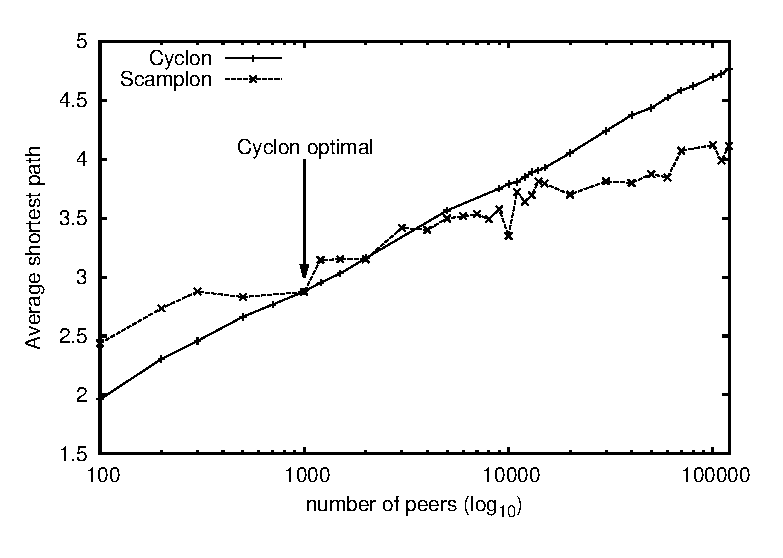
\includegraphics[width=0.49\textwidth]{img/avgpath.eps}
  \caption{\label{fig:avgpath}The average shortest path in \SPRAY and
    \CYCLON. The x-axis denotes the $\log_{10}$-scaled number of peers in the
    network while the y-axis denotes the average shortest path length of the
    network.}
\end{figure}

\subsection{In-degree distribution}
\label{subsec:dist}

\begin{figure}
  \centering
  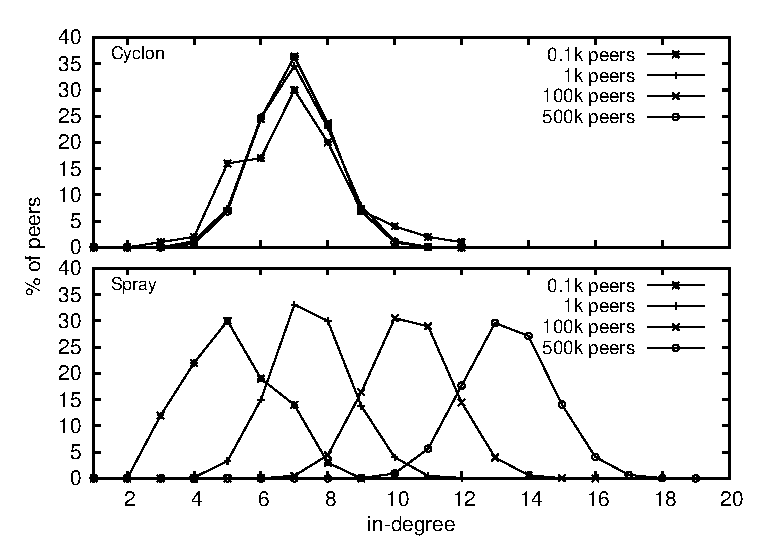
\includegraphics[width=0.49\textwidth]{img/histo.eps}
  \caption{\label{fig:histo}The in-degree distribution of \CYCLON and
    \SPRAY. The x-axis denotes the in-degree in number of nodes while the
    y-axis indicates the percentage of peers with such in-degree. The top
    figure is dedicated to the runs concerning \CYCLON while the bottom figure
    concerns \SPRAY.}
\end{figure}


\begin{figure*}
  \centering
  \subfloat[Figure A][\label{fig:churnA}The x-axis denotes the
  elapsed time in cycles. The upper graph y-axis shows the number of total
  connections in the overlay while the lower graph y-axis shows the variance
  $\sigma^2$ of the partial view sizes in the network.]{
    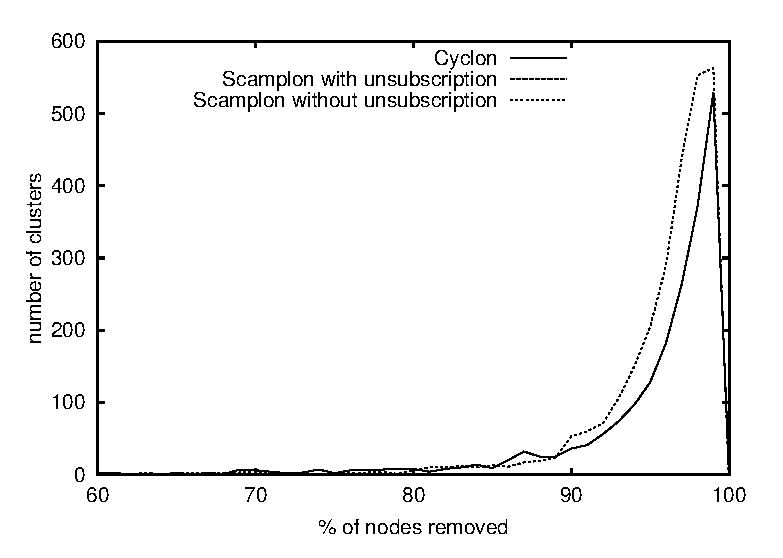
\includegraphics[width=0.45\textwidth]{img/churn.eps}}
  \hspace{10pt}
  \subfloat[Figure B][\label{fig:churnB}The x-axis denotes the
  elapsed time in cycles. The y-axis denotes the average partial view size.]{
    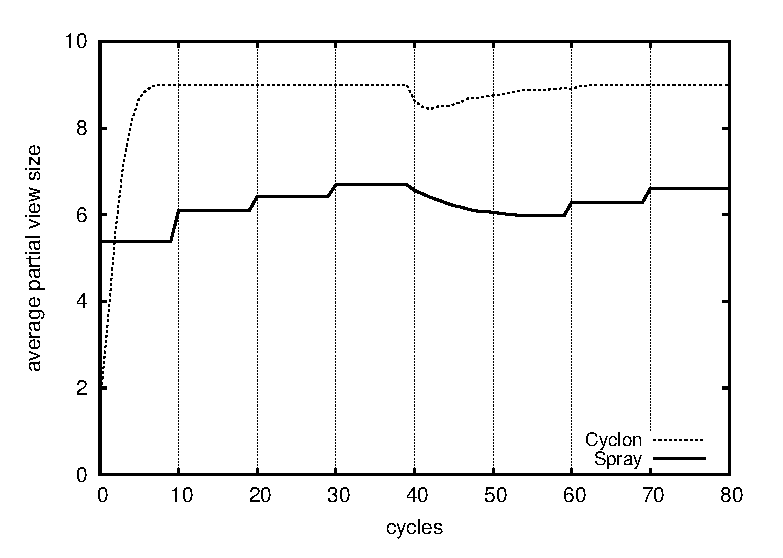
\includegraphics[width=0.45\textwidth]{img/avgpv.eps}}
  \caption{\label{fig:churn}\CYCLON (partial view size configured to 9) and
    \SPRAY in a dynamic network. 2.5k peers join the network at cycles $0$,
    $10$, $20$, and $30$. Then 5k peers leave at cycle $40$. Finally 2.5k peers
    join at cycles $60$ and $70$. The final network contains 10k members.}
\end{figure*}


\begin{asparadesc}
\item[Objective:] To observe how adaptiveness impacts the in-degree
  distribution, i.e., the load-balancing among peers.
\item[Description:] The in-degree of a peer shows how well this peer is
  represented in others' partial view. The in-degree distribution of the
  network can highlight the existence of weakly connected peers and/or strongly
  connected hubs. It has a direct impact on robustness. In this experiment, the
  fixed-size partial view approach is \CYCLON{}. It is configured with partial
  views of size $7$ which is optimal for a network of roughly $1100$ peers.
  For all the experiments, we perform the in-degree measurements after
  convergence. The measurements concern networks with 0.1k, 1k, 100k, 500k
  peers.
\item[Results:] Figure~\ref{fig:histo} shows the in-degree distribution of
  \CYCLON and \SPRAY. In the top figure, we observe that the distribution and
  the degrees of \CYCLON are identical, independently of the network
  size. Thus, the distribution of 0.1k peers is identical to the 500k one with
  a mean value of roughly 7 with a strong peak on this value. On the other
  hand, the bottom figure shows that the distribution of \SPRAY follows average
  partial view size which follows the network size
  growth. Figure~\ref{fig:histo} also shows that peers are very gathered around
  the mean partial view size. For instance, for the run with 500k peers using
  \SPRAY, the mean value for the in-degree is 13.37 and 88 percents of the
  peers have an in-degree comprised between 12 and 14 included. It means that
  the load is well balanced among peers. Since peers are equally important in
  term of connectedness, the network is robust to failures.
\item[Reasons:] Once configured, \CYCLON must handle any number of peers in the
  network with a fixed-size partial view. Proportionally, the number of times
  that a particular peer is referenced does not change compared to the network
  size. Indeed, the number of arcs that a new peer brings to network when it
  joins constitutes that many arcs targeting it after the shuffling
  rounds. Since the partial view size is constant, the in-degree of peers stays
  stable. On the other hand, in \SPRAY, each joining peer brings a increasing
  number of arcs in the network. Thus, the in-degree of each peer grows
  reflecting the network size. Hence, the distribution in the bottom figure
  shifts slowly to higher in-degree values as the network size grows.  \SPRAY
  does not peak on a particular value as \CYCLON because the average partial
  view size for a particular network size falls in-between integer values. For
  instance, if the average partial view size is 6.5, then half of them will
  have a size of 6 while the other half will have a size of 7. Such network is
  robust to failure because no peer is more important than other in term of
  connectedness. Therefore, if some random peer crashes, it will not affect as
  much the network as if a peer strongly connected crashed.
\end{asparadesc}

\subsection{Dynamic network}

% \begin{figure}
%   \centering
%   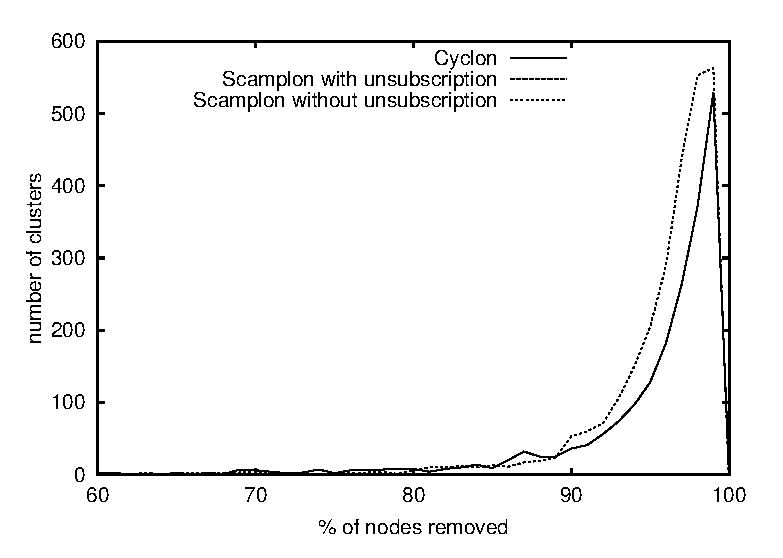
\includegraphics[width=0.49\textwidth]{img/churn.eps}
%   \caption{\label{fig:churn}\SPRAY in a dynamic network. The x-axis denotes
%   the elapsed time in cycles. The upper graph y-axis shows the number of
%   total connections in the overlay while the lower graph y-axis shows the
%   variance $\sigma^2$ of the partial view sizes $|\mathcal{P}|$ in the
%   network.  2.5k peers join the network at cycles $0$, $10$, $20$, and
%   $30$. Then 5k peers leave at cycle $40$. Finally 2.5k peers join at cycles
%   $60$ and $70$. The final network contains 10k members.}
% \end{figure}

\begin{asparadesc}
\item[Objective:] To show the impact of adaptiveness when the network size
  changes over time.
\item[Description:] In this experiment we focus on a dynamic network where
  peers can join and leave. The runs involve \CYCLON and \SPRAY. The \CYCLON's
  configuration targets roughly 8.1k peers. Thus, it is oversized compared the
  network size during the simulation (maximum 1k peers). During the first half
  of the experimentation, 250 peers are added 4 times successively by intervals
  of 10 cycles each. Thus, the network size goes from 0 to 1k peers in 40
  rounds. Then, half of the network leaves without giving notice (500
  peers). Finally, 250 peers join two additional times. The final network
  contains 1k members. The measurements concern
  \begin{inparaenum}
  \item the number of connections in the network over cycles,
  \item the variance of the partial view sizes over cycles
    (cf. Section~\ref{subsec:cyclic}),
  \item the average partial view size of peers.
  \end{inparaenum}
\item[Results:] Figure~\ref{fig:churn} shows the result of the experiment. The
  x-axis represents the cycles (i.e. the arbitrary unit time frame). The top
  part of Figure~\ref{fig:churnA} shows the number of connections established
  in the network (scale $\times 10^3$) while its bottom part shows the variance
  in the partial view size of the members. Concerning \SPRAY, we can see that
  at each batch of joinings, the connection number grows to reflect the needs
  of the new network membership. The observation is consistent with the
  variance measures. Indeed, at each batch of insertions, the variance suddenly
  grows. Then, it exponentially decreases and converges to zero in less than 10
  cycles. The variance is higher when the network size is lower. For instance,
  the first 250 peers lead to the highest variance. At the $40^{th}$ cycle,
  half of the peers leave/crash. Around half of the connections are directly
  removed without disturbing the variance of partial views. The 10 following
  cycles show a slight decrease of arcs. Then new members are introduced in the
  network yielding the same results as earlier joinings. \CYCLON exposes an
  identical behavior. Nevertheless, the number of arcs is invariably higher
  than the \SPRAY one (from 1000 to 2500 additional
  connections). Figure~\ref{fig:churnB} shows the average partial view size of
  \SPRAY and \CYCLON. As expected, \CYCLON immediately converges to the
  configured partial view size (9 neighbors). On the other hand, \SPRAY's
  partial views logarithmically grow while the network grows. When the removals
  occur at Cycle 40, the peers using \CYCLON remove the dead arcs while
  refilling their partial view until they reach the configured partial view
  size. \SPRAY only remove the arcs to reflect the departed peers. At the end,
  the \SPRAY partial views contain in average 6.6 neighbors (for the recall,
  $\ln(1000)\approx 6.9$).
\item[Reasons:] Since the partial views of \SPRAY adapt themselves to the
  network size, the number of connections grows as the network membership
  grows.  The peaks in variance correspond to the joining parts of the
  experiment. The disparity comes from the fact that new peers arrive in the
  network with a small partial view. The peaks are smaller when the network is
  larger. Indeed, the peers - which already were network members before the new
  arrivals - had a few cycles to exchanges and even up their partial views. As
  consequence, it lessens the weight of joinings. The removal of 500 peers does
  not disturb the variance since each crashing/leaving peer is chosen at
  random. Thus, no peers suffer more of these removals than others. The
  slightly decreasing number of arcs after the removal is due to peers
  realizing that some arcs are dead, leading to a probabilistic removal
  (cf. Algorithm~\ref{algo:unreachable}). 
\end{asparadesc}

\subsection{Massive failures}
\label{subsec:resilience}

\begin{figure}
  \centering
  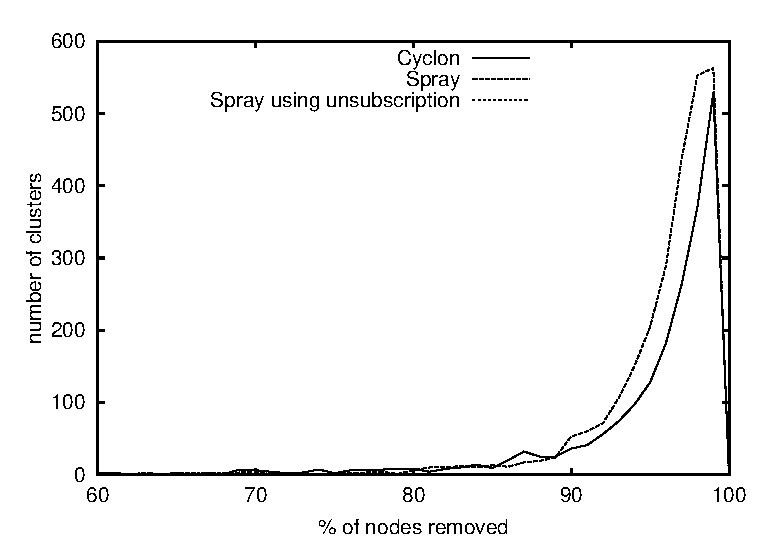
\includegraphics[width=0.49\textwidth]{img/resilience.eps}
  \caption{\label{fig:resilience}Robustness of \CYCLON and \SPRAY to massive
    failures. The x-axis denotes the percentage of peers removed at once in a
    network containing 10k members. The y-axis denotes the number of
    components over the current network size (after the removals). The
    measurements concern the weak and strong components which basically means
    the number clusters in undirected or directed graph respectively.}
\end{figure}

% \begin{algorithm}
% 
\small
\algrenewcommand{\algorithmiccomment}[1]{\hskip2em$\rhd$ #1}

\newcommand{\comment}[1]{$\rhd$ #1}

\algblockdefx[initially]{initially}{endInitially}
  [0] {\textbf{INITIALLY:}}

\algblockdefx[pas]{pas}{endPas}
  [0] {\textbf{EVENTS:}}

\newcommand{\LINEFOR}[2]{%
  \algorithmicfor\ {#1}\ \algorithmicdo\ {#2} %
  }

\newcommand{\LINEIFTHEN}[2]{%
  \algorithmicif\ {#1}\ \algorithmicthen\ {#2} %
  }

\newcommand{\INDSTATE}[1][1]{\State\hspace{\algorithmicindent}}

\begin{algorithmic}[1]
  \Statex
  \initially
  \State $\mathcal{I}$ \hfill \label{line:inview}
  \comment{set of peers targeting us ($p$) in their partial view}
  \endInitially

  \pas
    \Function{unSubscribe}{\ }
    \For{$i\leftarrow 0$ \textbf{to} $min(|\mathcal{P}|,\, |\mathcal{P}|-1)$ 
      \label{line:bridge}}    
    \State \textbf{let} $\langle n,\,\_ \,\rangle \leftarrow \mathcal{P}[i]$;
    \State $sendTo(\, \mathcal{I}[\,i\%|\mathcal{I}|\,],\, 'unSubs',\, n)$;
    \EndFor
    \EndFunction
    \Statex
    \Function{onUnSubs}{$o, \, n$} 
    \hfill \comment{$o$: origin; $n$: neighbor to add}
    \State $\mathcal{P}\leftarrow (\mathcal{P}\setminus o)
    \uplus\{\langle n,\,0\rangle\}$;
    \EndFunction
  \endPas
\end{algorithmic}

% \caption{\label{algo:unsubscription}Unsubscription protocol from
%   \SCAMP~\cite{ganesh2003peer}}
% \end{algorithm}

\begin{asparadesc}
\item[Objective:] To show that both \SPRAY and \CYCLON are equally robust to
  massive failures.
\item[Description:] Counting the strong components in a network allows
  estimating the area that are reachable by the information dissemination
  protocols. For instance, there are 2 strong components if a part of the
  network can reach another part and the converse being false.  Counting the
  weak components in a network allows estimating the point where the network is
  still in a repairable state, i.e., after some shufflings, the network will
  converge to an overlay where the information dissemination is able to reach
  all members again. \CYCLON has a partial view size set to 9. The network
  contains 10k members. We perform the removals after the approaches converged
  to a stable overlay network. We remove the batch of peers at once, from 25 to
  95 percents of peers every 5 percents, i.e., 16 runs for each approach. We
  perform a last measurement at 99 percents. We perform the measurements
  immediately after the removals. The removals concern a percentage of the
  peers chosen at random among the 10k members.
\item[Results:] Figure~\ref{fig:resilience} shows the ratio of strong/weak
  components over the network size after removals. Firstly, the figure shows
  that both the random peer sampling protocols \SPRAY and \CYCLON suffer from
  deteriorated behavior at high removal percentages, \CYCLON being slightly
  better in this term. Figure~\ref{fig:resilience} shows that the information
  dissemination (strong components) starts to slowly degrade at 45 percents,
  and quickly degrade at 70 percents. Fortunately, Figure~\ref{fig:resilience}
  also shows that the approaches are able to recover from such clustering until
  high removal rate. Indeed, the weak components start to increase at 70
  percents. Meaning that some part of the network are completely disjoint and
  beyond repair.
\item[Reasons:] The random peer sampling approaches \CYCLON and \SPRAY expose
  very similar results because \CYCLON's configuration targets a network size
  of 10k peers, while \SPRAY adjusts itself automatically to this network size.
  Therefore, the arcs number in the approaches are close from being identical
  \CYCLON is slightly better because, in this case, it has more arcs (due to
  \SPRAY's randomness) and because it does not have duplicates (\SPRAY contains
  a small amount of duplicates in the partial view,
  cf. Section~\ref{subsec:duplicates}). It requires a high amount of removals
  to endanger the information dissemination protocol's ability to reach all
  peers. Indeed, since all peers are equally important in the network
  (cf. Figure~\ref{fig:histo}), removing a particular peer does not greatly
  affect the whole network. The network membership protocol is able to repair
  the topology later than the information dissemination starts to fail because
  the direction of arcs is not as important as in the latter. Indeed, \CYCLON
  and \SPRAY are still able to repair a network until parts of the network
  become disjoint, i.e., there is no arc between these parts of the network.
\end{asparadesc}

\subsection{Duplicates in partial views}
\label{subsec:duplicates}

\begin{figure}
  \centering
  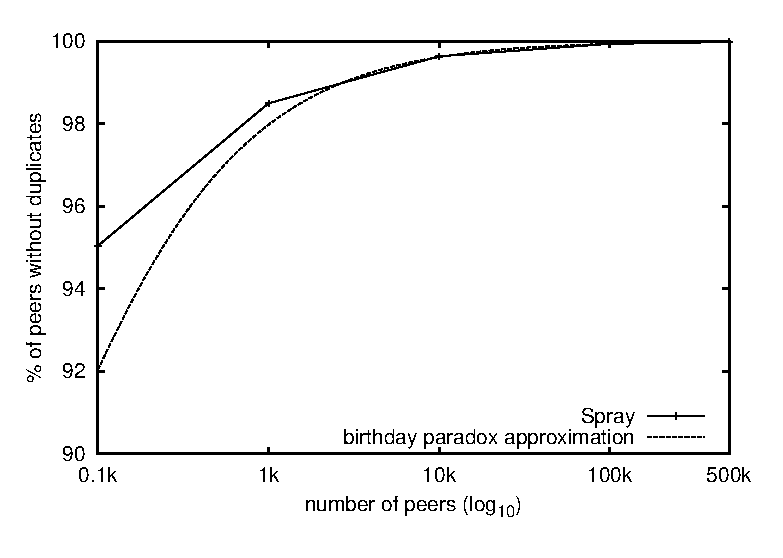
\includegraphics[width=0.49\textwidth]{img/duplicates.eps}
  \caption{\label{fig:duplicates}Duplicates in networks of different size: the
    $\log_{10}$-scaled x-axis denotes the network size while y-axis denotes the
    proportion of peers without any duplicates in their partial view.}
\end{figure}

\begin{asparadesc} 
\item[Objective:] To show that the number of peer containing duplicates in
  their partial view is always low.  To show that this proportion becomes minor
  in large networks. To highlight the relation between the birthday paradox and
  the proportion of duplicates.
\item[Description:] Using \SCAMP as random peer sampling protocol, we measure
  the amount of peers which have a partial view containing at least one
  duplicated reference. We perform the measurements on networks containing
  0.1k, 1k, 10k, 100k, and 500k peers. We measure the number of duplicates
  after convergence. We put this in relation with a theoretical approximation
  from the birthday paradox. The probability of a peer to not have duplicates
  is approximately:
  \begin{equation}
    1- 
    (1-
    \exp({-\ln(|\mathcal{N}|)*(\ln(|\mathcal{N}|)-1)\over{2*|\mathcal{N}|}}))
  \end{equation}
\item[Results:] Figure~\ref{fig:duplicates} shows the proportion of peers using
  a partial view containing duplicates. As we can observe, there always exist
  partial views with at least one duplicate. The proportion is more important
  when the network size is small (e.g. 5 percents for 0.1k peers), and it
  becomes a minor overhead when the network size is larger (e.g. less than 1
  percent for 10k peers). The birthday paradox approximation seems to follow
  very closely the experimental results. It empirically confirms that there
  exist a relation between the duplicates and the birthday paradox. The
  proportion of peers without duplicates tends to 100 percents as the network
  size grows.
\item[Reasons:] As the network grows, the chances of a particular peer to have
  at least twice the reference to another peer becomes smaller. Indeed, while
  the network grows linearly, the number of references to a particular peer
  only grows logarithmically. Nevertheless, the birthday paradox reminds that
  this proportion is not as small as it seems to be.
\end{asparadesc}


\subsection{Failures in connection establishment}
\label{subsec:degeneration}

\begin{figure}
  \centering 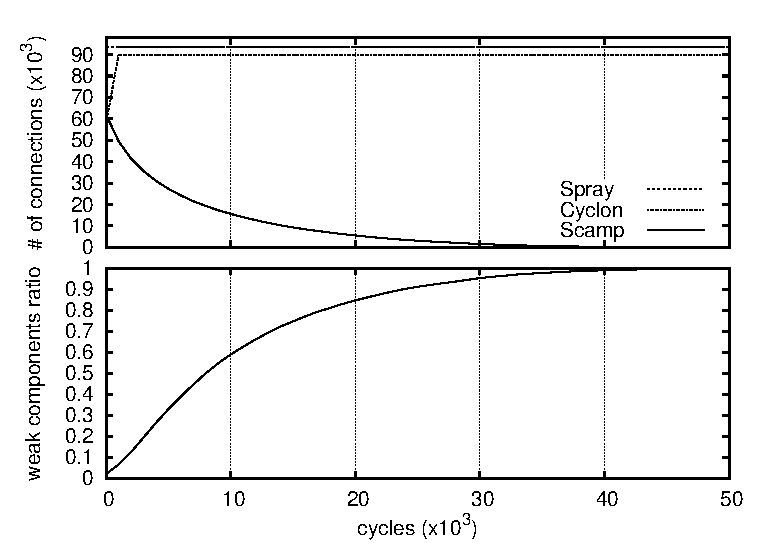
\includegraphics[width=0.49\textwidth]{img/degen.eps}
  \caption{\label{fig:degeneration}\CYCLON, \SCAMP, and \SPRAY in network
    subject to failures in the connection establishments. The x-axis denotes
    the elapsed time in cycles ($10^3$-scaled). The y-axis of the top figure
    denotes the global number of arcs ($10^3$-scaled). The y-axis of the bottom
    figure denotes the ratio of weak components over the current network size.}
\end{figure}

\begin{asparadesc}
\item[Objective:] To show that \SPRAY does not suffer from failures in
  connection establishments, contrarily to \SCAMP.
\item[Description:] We measure both the arcs count and the number of weak
  components in the network. The simulations involve \CYCLON configured with
  partial view containing 9 neighbors (targeting a network of roughly 8100
  peers), \SCAMP\footnote{A modified version of \SCAMP whose periodic protocol
    works properly when there is no connection failures. Available at
    \url{https://github.com/justayak/peersim-spray}}, and \SPRAY, running over
  70k cycles. The network initially contains 10k members. The probability that
  a message fails to arrive to its destination (each hop) is set to $10^-3$. To
  establish a connection, we use the WebRTC three-way handshake, i.e., the
  initial peer emits an offer ticket, the arrival peer stamps the ticket, the
  initial peer finalizes the connection using the stamped ticket
  (cf. Section~\ref{sec:relatedwork}).
\item[Results:] Figure~\ref{fig:degeneration} is comprised of two parts. The
  top figure shows the arc count of the random peer samplings while the bottom
  figure shows the weak components of the network.  First, we observe that, as
  expected, the arc count of \CYCLON and \SPRAY stays constant over cycles: 90k
  and 93k arcs for \CYCLON and \SPRAY respectively. Second, we observe that
  \SCAMP suffers from the failures on connection establishments. It directly
  impacts on the connectedness of the network represented by the weak
  components ratio. The network of \SCAMP quickly degrades.
\item[Reasons:] The arc count of both \CYCLON and \SPRAY remains constant over
  time but for different reasons. In \CYCLON, the shuffling protocol makes sure
  that the partial view is filled to its maximum. Thus, when it uses a not
  successfully established connection to perform an exchange, it simply
  discards the connection, knowing that the next exchange is likely to overfill
  its partial view. In \SPRAY, when a connection fails to establish and the
  protocol tries to use it for an exchange, it will replace this arc with
  another known reference. Thus, the arc count stays constant and the shuffling
  protocol makes sure that duplicates disappear over time (the arc moves to
  another peer where it is not a duplicate). In \SCAMP, the connections are
  much more likely to fail than in the aforementioned protocols. Indeed,
  contrarily to these latter, \SCAMP does not cautiously establish connections
  with the neighbors of its neighbors.  Each hop of its ticket dissemination is
  an opportunity of failure. Since there is no routing in such network, the
  only way for a stamped ticket to come back to its emitter is the path it
  traveled in the first place. Hence, all peers belonging to the path must stay
  alive until the stamped ticket comes back in order to consistently forward
  it.  Furthermore, its periodic protocol starts with an immediate cutting of
  the incoming arcs of the initiating peer because it assumes that the new
  connections spread in the network will establish.  Since it does not, the
  peer eventually becomes disconnected. Also, when its neighbors execute the
  periodic protocol, they delete their reference in its partial view. In such
  case, the peer becomes disconnected.  Hence the quick degeneration of the
  \SCAMP arc count. Hence the quick partitioning of the network.
\end{asparadesc}


%%% Local Variables:
%%% mode: latex
%%% TeX-master: "../paper"
%%% End:
